\section{Volumenkontrol}

\begin{frame}{Volumenkontrol - Krav}
\scriptsize{
\begin{table}[h]
\centering
\begin{tabular}{l|r}
\hline\hline
Område & Krav \\
\hline\hline
Frekvensgang & \< 0,375 dB ved 20 Hz - 20 kHz, ref. 1 kHz \\
& \< 0,75 dB fra 20 Hz til 63 Hz \\
& \< 0,75 dB fra 12,5 kHz til 20 kHz \\[4pt]
Dæmpningsområde i & 0 - 50 dB ved 1 kHz \\
volumenkontrol & \\[4pt]
Styring af volumen- & Digital \\
kontrol & \\[4pt]
Antal niveauer i & 51 \\
volumenkontrollen & \\[4pt]
Dæmpning per & 1 dB \\
niveau & \\[4pt]
Input fra brugeren & To trykknapper \\[4pt]
Output til brugeren & To 7-segmenter \\
\hline\hline
\end{tabular}
%\caption{Krav til volumenkontrollen}
%\label{tab:krav_volumenkontrol}
\end{table}}
\end{frame}

\begin{frame}{Volumenkontrol - Alternativer}
\begin{itemize}
\item Potentiometer
\item Processor
\end{itemize}
\end{frame}

\begin{frame}{Volumenkontrol - Blokdiagram}
\begin{figure}[h]
\centering
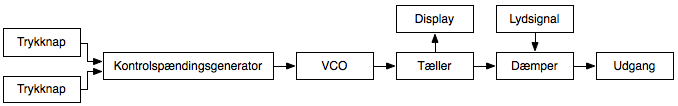
\includegraphics[scale=0.4]{images/blokdiagram-volumenkontrol.png}
%\caption{Overordnet blokdiagram over volumenkontrollen}
%\label{fig:blokdiagram_volumenkontrol}
\end{figure}

\begin{itemize}
\item Kontrolspændingsgenerator
\item VCO
\item Tæller
\item Display
\item Dæmper
\end{itemize}
\end{frame}

\begin{frame}{Volumenkontrol - Brug}
\begin{figure}[h]
\centering
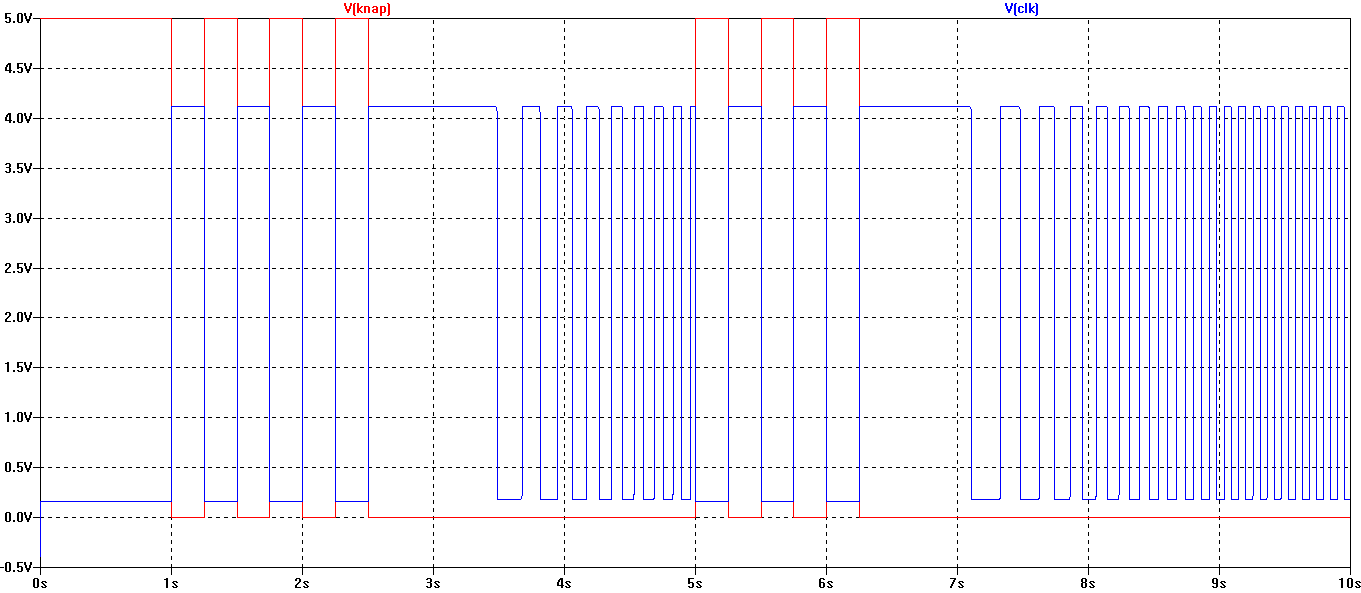
\includegraphics[scale=0.285]{images/volumenkontrol-test.png}
\end{figure}
\end{frame}

\begin{frame}{Volumenkontrol - Frekvensgang - Niveau 0}
\begin{figure}[h]
\centering
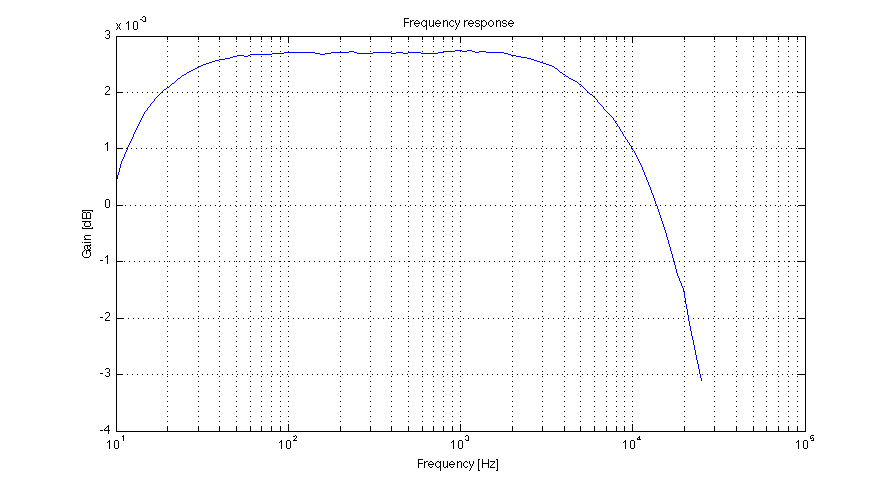
\includegraphics[scale=0.3]{images/2Vniveau0-frek.png}
\end{figure}
\scriptsize{
\begin{table}[h]
\centering
\begin{tabular}{l|r|r}
\hline\hline
Område & Krav & Status \\
\hline\hline
Frekvensgang & \< 0,375 dB ved 20 Hz - 20 kHz, ref. 1 kHz & \checkmark \\
& \< 0,75 dB fra 20 Hz til 63 Hz & \checkmark \\
& \< 0,75 dB fra 12,5 kHz til 20 kHz & \checkmark \\[4pt]
Dæmpning per & 1 dB & \checkmark \\
niveau && \\[4pt]
\hline\hline
\end{tabular}
\end{table}}
\end{frame}

\begin{frame}{Volumenkontrol - Frekvensgang - Niveau 25}
\begin{figure}[h]
\centering
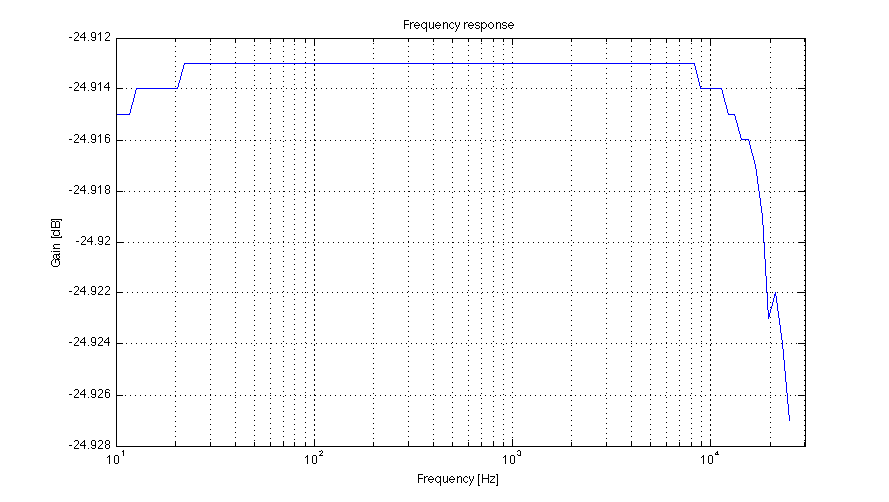
\includegraphics[scale=0.3]{images/2Vniveau25-frek.png}
\end{figure}
\scriptsize{
\begin{table}[h]
\centering
\begin{tabular}{l|r|r}
\hline\hline
Område & Krav & Status \\
\hline\hline
Frekvensgang & \< 0,375 dB ved 20 Hz - 20 kHz, ref. 1 kHz & \checkmark \\
& \< 0,75 dB fra 20 Hz til 63 Hz & \checkmark \\
& \< 0,75 dB fra 12,5 kHz til 20 kHz & \checkmark \\[4pt]
Dæmpning per & 1 dB & \checkmark \\
niveau && \\[4pt]
\hline\hline
\end{tabular}
\end{table}}
\end{frame}

\begin{frame}{Volumenkontrol - THD}
\begin{figure}[h]
\centering
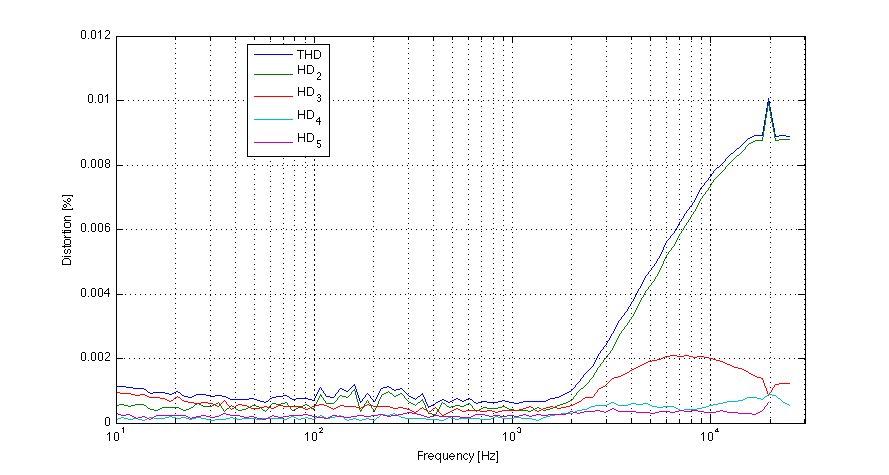
\includegraphics[scale=0.4]{images/2Vniveau0-thd.png}
\end{figure}
\end{frame}

\begin{frame}{Volumenkontrol - Accepttest}
\scriptsize{
\begin{table}[h]
\centering
\begin{tabular}{l|r|r}
\hline\hline
Område & Krav & Status \\
\hline\hline
Frekvensgang & \< 0,375 dB ved 20 Hz - 20 kHz, ref. 1 kHz & \checkmark \\
& \< 0,75 dB fra 20 Hz til 63 Hz & \checkmark \\
& \< 0,75 dB fra 12,5 kHz til 20 kHz & \checkmark \\[4pt]
Dæmpningsområde i & 0 - 50 dB ved 1 kHz & \checkmark \\
volumenkontrol && \\[4pt]
Styring af volumen- & Digital & \checkmark \\
kontrol && \\[4pt]
Antal niveauer i & 51 & $\mathcal{X}$ \\
volumenkontrollen && \\[4pt]
Dæmpning per & 1 dB & \checkmark \\
niveau && \\[4pt]
Input fra brugeren & To trykknapper & \checkmark \\[4pt]
Output til brugeren & To 7-segmenter & \checkmark \\
\hline\hline
\end{tabular}
%\caption{Oversigt over status af krav til volumenkontrollen}
%\label{tab:krav_volumenkontrol}
\end{table}}
\end{frame}